\ylDisplay{Plokk} % Ülesande nimi
{Tundmatu autor} % Autor
{lahtine} % Voor
{2006} % Aasta
{G 5} % Ülesande nr.
{5} % Raskustase
{
% Teema: Dünaamika
\ifStatement
Kui suure kiirendusega $a_k$ ja mis suunas hakkab liikuma kahest kehast koosneva süsteemi masskese, kui kehad on seotud niidiga, mis on tõmmatud üle ploki (vt joonist)? Kehade massid on $m_1$ ja $m_2$ ($m_1$ < $m_2$), niit on kaalutu ja mitteelastne.
\begin{center}
	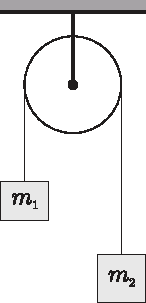
\includegraphics[width=0.25\linewidth]{2006-lahg-05-yl}
\end{center}
\fi


\ifHint
Ülesandes niidi pinge $T$ teada, aga see on leitav pannes plokkide jaoks kirja Newtoni teise seaduse ning niidi venimatuse tingimuse. Massikeskme kiirenduse avaldamine plokkide kiirenduste kaudu on analoogne massikeskme koordinaadi avaldamisega plokkide koordinaatide kaudu.
\fi


\ifSolution
Kuna raskem keha hakkab liikuma allapoole ja kergem ülespoole, siis on selge, et süsteemi massikese hakkab liikuma allapoole. 

Olgu süsteemi massikese alghetkel punktis $C_0$ (vt joonist). Kehade massikeskmete kaugused süsteemi massikeskmest leiame tingimusest: 
\begin{equation} \label{2006-lahg-05:eq1}
m_1b_1 = m_2b_2.
\end{equation}
Aja $t$ jooksul raskem keha liigub allapoole ja kergem liigub ülespoole kauguse $H$ võrra:

\begin{center}
	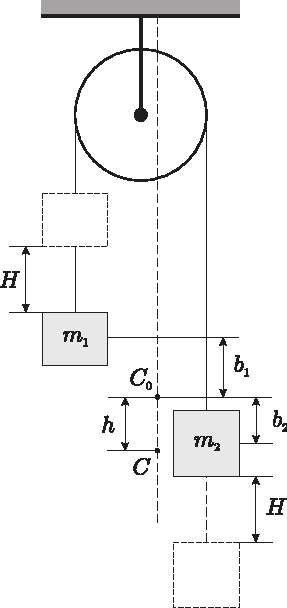
\includegraphics[width=0.4\linewidth]{2006-lahg-05-lah}
\end{center}

\begin{equation} \label{2006-lahg-05:eq2}
H = at^2 2,
\end{equation}
kus $a$ on kehade kiirendus. Süsteemi masskese liigub sama aja jooksul kauguse $h$ võrra, mille määrab tingimus:
\[
m_2 (H + b_2 - h) = m_1 (H + b_1 + h).
\]
Siit, arvestades valemeid (\ref{2006-lahg-05:eq1}) ja (\ref{2006-lahg-05:eq2}), leiame, et:
\begin{equation} \label{2006-lahg-05:eq3}
h=\frac{m_{2}-m_{1}}{m_{2}+m_{1}} H=\frac{m_{2}-m_{1}}{m_{2}+m_{1}} \frac{a t^{2}}{2}.
\end{equation}
Kiirenduse $a$ leiame võrrandisüsteemist: 
\[
m_2a = m_2g - T,\quad m_1a = T - m_1g,
\]
kus $T$ on niidi tõmbepinge. Avaldades $a$ võrrandisüsteemist, saame
\[
a=\frac{m_{2}-m_{1}}{m_{2}+m_{1}} g.
\]
Asendades leitud väärtuse valemisse (\ref{2006-lahg-05:eq3}), saame:
\[
\begin{aligned}
h&=\left(\frac{m_{2}-m_{1}}{m_{2}+m_{1}}\right)^{2} \frac{g t^{2}}{2}=\frac{a_{k} t^{2}}{2} \quad \Rightarrow \\ 
&\Rightarrow \quad a_{k}=\left(\frac{m_{2}-m_{1}}{m_{2}+m_{1}}\right)^{2} g.
\end{aligned}
\]
\fi
}